\documentclass{beamer}
\usepackage{inconsolata}
\usepackage{color}
\usepackage{listings}
\usepackage{cooltooltips}
\usepackage{hyperref}
\usepackage[normalem]{ulem}
\setbeamertemplate{navigation symbols}{}%remove navigation symbols
\usepackage{listings}
\usepackage{color}
\usepackage{framed}

\definecolor{background}{RGB}{39, 40, 34}
\definecolor{string}{RGB}{230, 219, 116}
\definecolor{comment}{RGB}{117, 113, 94}
\definecolor{normal}{RGB}{248, 248, 242}
\definecolor{identifier}{RGB}{166, 226, 46}



\lstset{
  language=C,               			% choose the language of the code
  alsolanguage=Python,            			% choose the language of the code
  alsolanguage=Java,            			% choose the language of the code
  numbers=none,                   		% where to put the line-numbers
  stepnumber=1,                   		% the step between two line-numbers.        
  numbersep=5pt,                  		% how far the line-numbers are from the code
  extendedchars=true,
  numberstyle=\tiny\color{black}\ttfamily,
  backgroundcolor=\color{background},  		% choose the background color. You must add \usepackage{color}
  showspaces=false,               		% show spaces adding particular underscores
  showstringspaces=false,         		% underline spaces within strings
  showtabs=false,                 		% show tabs within strings adding particular underscores
  frame=single,
  framerule=0pt,
  tabsize=4,                      		% sets default tabsize to 2 spaces
  captionpos=n,                   		% sets the caption-position to bottom
  breaklines=true,                		% sets automatic line breaking
  breakatwhitespace=true,         		% sets if automatic breaks should only happen at whitespace
  title=\lstname,                 		% show the filename of files included with \lstinputlisting;
  basicstyle=\color{normal}\tiny\ttfamily,					% sets font style for the code
  keywordstyle=\color{magenta}\tiny\ttfamily,	% sets color for keywords
  stringstyle=\color{string}\tiny\ttfamily,		% sets color for strings
  commentstyle=\color{comment}\tiny\ttfamily,	% sets color for comments
  emph={True, False, format_string, eff_ana_bf, permute, eff_ana_btr, KeyError,
  ValueError, ZeroDivisionError},
  emphstyle=\color{identifier}\tiny\ttfamily,
  morekeywords={with, as}
}

\lstset{literate=%
   *{0}{{{\color{cyan}0}}}1
    {1}{{{\color{cyan}1}}}1
    {2}{{{\color{cyan}2}}}1
    {3}{{{\color{cyan}3}}}1
    {4}{{{\color{cyan}4}}}1
    {5}{{{\color{cyan}5}}}1
    {6}{{{\color{cyan}6}}}1
    {7}{{{\color{cyan}7}}}1
    {8}{{{\color{cyan}8}}}1
    {9}{{{\color{cyan}9}}}1
}



\hypersetup{
  colorlinks=true,
  urlcolor=pink,
}

\title{Python 101}
\subtitle{Lec03 \\ Functions}
\author{thoum}

\begin{document}
\frame{\titlepage}

\begin{frame}
\frametitle{Functions}
  $$f(x) = x+1$$
  $$f(x) = \ln x$$
  %Fibonacci.
  %$$f(x) = f(x-1) + f(x-2)$$
\end{frame}

\begin{frame}[fragile]
\frametitle{Python Functions}
\begin{lstlisting}
def f(x):
    r = x+1
    return r

def g(x):
    return math.log(x)

#Note that each x is unique to the function

print(f(3)) # f(3) becomes 3+1
print(f(3))
\end{lstlisting}
\end{frame}
\begin{frame}
\frametitle{Why Functions?}
  \begin{itemize}
    \item Reusability
    \item Abstraction
    \item And many more
  \end{itemize}
\end{frame}

\begin{frame}
\frametitle{Reusability}
  \begin{lstinputlisting}
    {./not_reuse.py}
  \end{lstinputlisting}
\end{frame}

\begin{frame}
\frametitle{Reusability}
  \begin{lstinputlisting}
    {./reusability.py}
  \end{lstinputlisting}
\end{frame}

\begin{frame}
\frametitle{Reusability}
\begin{itemize}
  \item Less code to read
  \item Fix once, fix everywhere
\end{itemize}
\end{frame}

\begin{frame}[fragile]{Abstraction}
  \begin{lstlisting}
print()
  \end{lstlisting}
  vs
  \begin{lstinputlisting}
    {./print_code.c}
  \end{lstinputlisting}
\end{frame}

\begin{frame}{Abstraction}
  \begin{itemize}
    \item Lets us focus
  \end{itemize}
\end{frame}

\begin{frame}{Understanding Functions}
  Some functions(\textit{pure} functions) are just values
  \begin{lstinputlisting}
    {./pure_function.py}
  \end{lstinputlisting}
\end{frame}

\begin{frame}{Understanding Functions}
  Some functions have side effects
  \begin{lstinputlisting}
    {./side_effect.py}
  \end{lstinputlisting}
\end{frame}

\begin{frame}{Understanding Functions}
  Some functions have side effects (cont'd)
  \begin{lstinputlisting}
    {./side_effect2.py}
  \end{lstinputlisting}
\end{frame}

\begin{frame}{Detour: Wait..What just happened?}
  Function parameters can be thought as names or labels (in python).\\

  Imagine that function is a dark room.\\
  We can only interact with outer objects that enters this room by 
  giving them \textcolor{green}{glow-in-the-dark} stickers with their names on it.
\end{frame}

\begin{frame}[fragile]{Detour: Wait..What just happened?}
  Here, we gave outer $x$ the sticker that says l.

  By l[0], we were able to reach x[0].
  \begin{lstlisting}
x = [1,2,3]
def change_element_of_list(l):
    l[0] = 3
change_element_of_list(x)
print(x)
  \end{lstlisting}
\end{frame}

\begin{frame}[fragile]{Detour: Wait..What just happened?}
  When we $l = 2$, we took the sticker from $x$ and gave it to $2$.\\
  Now, we can't see $x$ in the dark.

  \begin{lstlisting}
x = [1,2,3]
def change_without_global(l):
    print(l)
    l = 2
change_without_global(x)
print(x)
  \end{lstlisting}
\end{frame}

\begin{frame}[fragile]{Detour: Wait..What just happened?}
  Using $global$ is like giving a permanent sticker to $y$, with name $y$ written
  on it.
  \begin{lstlisting}
y = [1,2,3]
def change_by_global():
    global y
    y = 3
print(y)
  \end{lstlisting}
\end{frame}

\begin{frame}{Detour: Wait..What just happened?}
  Confusing? 
  Good news: We will get used to it.\\
  Bad news: Side effects are inevitable.\\
  So let's try our best to keep it to a minimum.

  \href{https://stackoverflow.com/questions/575196/why-can-a-function-modify-some-arguments-as-perceived-by-the-caller-but-not-oth}{Click
  for details.}
\end{frame}

\begin{frame}{Function Practice}
  Choose any code we have written (giving grades? printing stars? is
  string a palindrome?) and turn it to a function.
\end{frame}

\begin{frame}{Recursion}
  What is recursion?  It is...
\end{frame}

\begin{frame}{Recursion}
  What is recursion?  It is...
\end{frame}

\begin{frame}{Recursion}
  What is recursion?  It is...
\end{frame}

\begin{frame}{Recursion}
  What is recursion?  It is...
\end{frame}

\begin{frame}{Recursion}
  
\includegraphics[width=100mm]{./recursion.png}
\end{frame}

\begin{frame}{Recursion}
  A thing is defined in terms of itself or of its type.
\end{frame}

\begin{frame}{Recursion????}
  What?
\end{frame}

\begin{frame}{Back to highschool}
  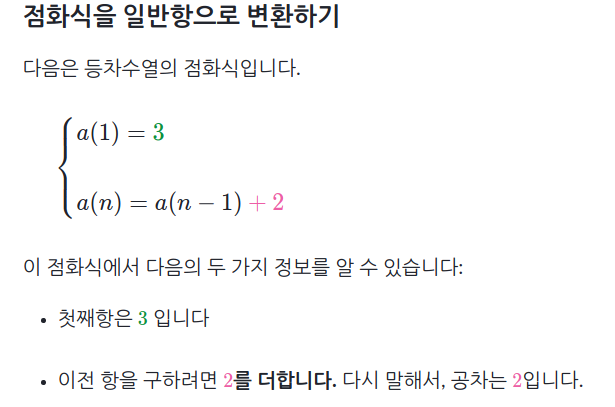
\includegraphics[width=100mm]{./jumhwasik.png}\\
  \href{https://ko.khanacademy.org/math/algebra/sequences/constructing-arithmetic-sequences/a/converting-recursive-and-explicit-formulas-of-arithmetic-sequences}{img
  source}
  
\end{frame}

\begin{frame}[fragile]{In Python}
  \begin{lstinputlisting}
    {./jumhwa.py}
  \end{lstinputlisting}
\end{frame}

\begin{frame}{In English}
  Assume $a(x)$ will somehow, magically calculate $a(n)$\\
  Then, just by writing out the definition, we are done.
\end{frame}

\begin{frame}{In Your Brain}
  Imagine what happens if we call $a(3)$.
  \begin{align*}
a(3) = &a(2) + 2\\
&a(2) = a(1) + 2\\
    &\phantom{{ab}={ab}} a(1) = a(0) + 2\\
    &\phantom{{ab}={ab}{ab}={ab}} a(0) = 3\\
    &\phantom{{ab}={ab}} a(1) = 5\\
    &a(2) = 7\\
a(3) = &9
  \end{align*}
  What if $a(0)$ is not defined?\\
\end{frame}

\begin{frame}{Importance of Base Case}
  $a(-1) \rightarrow a(-2) \rightarrow a(-3) ...$


  \textcolor{red}{Forever and ever and ever and ever and ever and ever and
  ever and ever and ever and ever and ever and ever and ever and ever and ever
  and ever and ever and ever and ever and ever and ever and ever and ever and
  ever and ever and ever and ever and ever and ever and ever and ever and ever
  and ever and ever and ever and ever and ever and ever and ever and ever and
  ever and ever and ever and ever and ever and ever and ever and ever and ever
  and ever and ever and ever}
  until we run out of memory.\footnote{Or not, look up
  \href{https://www.google.com/search?q=call+stack}{call stack} and
  \href{https://www.google.com/search?q=tail+call+optimization}{tail call
  optimization}}
\end{frame}

\begin{frame}{Recursion Practice}
  We used $for$ to implement the fibonacci sequence.
  Rewrite it using functions and recursion.\footnotemark[1]

  \footnotetext{Chruch-Turing thesis proves that this is $always$
  possible, given enough memory. \href{https://stackoverflow.com/questions/931762/can-every-recursion-be-converted-into-iteration}{Details
  here}}
\end{frame}

\begin{frame}{Solution}
  \begin{lstinputlisting}
    {./fib_rec.py}
  \end{lstinputlisting}
\end{frame}

\begin{frame}{Food for thought}
  Done?\\
  Does it print $fibonacci(10)$ well? What about $fibonacci(100)$?\\
  Compare it to the $for$ version. Why is it so slow? Try the $In Your Brain$
  exercise.
\end{frame}

\end{document}
